
\section{Simulation results}
We consider the worst case scenario of a prolonged energy crisis with $12$ cumulative shocks of $5\%$ ($d=240$, $\pi=0.05$, $\Pi=20$).
Figure \ref{Figure: energy shock 4 growth} shows the GDP growth rate during the energy crisis of the previous section. 

As discussed in the experimental design, we need to set the trigger for the policy.
The first trigger we set to $-5\%$, which means that the subsidy will not take effect until the annualized growth rate of GDP falls below $-5\%$. Note that the government in our model only detects this trigger once a year, so it really has to be a sustained economic downturn before the policy takes effect. In the example the subsidy would be activated around iteration 1200, when the economy first reaches below $-5\%$ growth.

The second trigger is set the $+5\%$ which in our example means that the subsidy would only be turned off at iteration 1600, when the economy starts to grow by more than $+5\%$ on a yearly basis. After that it never reaches below $-5\%$ again so the subsidy will remain inactive.

Figure \ref{Figure: Stabilization} shows the effect of the stabilizing subsidy. The growth rate is back to positive levels which is financed subsidy payments by the government.

\begin{figure}[ht!]
\centering\leavevmode
\begin{minipage}{17cm}
\centering\leavevmode
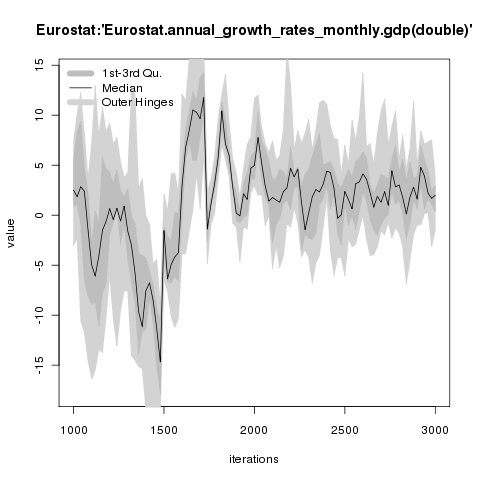
\includegraphics[width=8cm]{./energy_shock/png/duration_240/intensity_0.05/frequency_20/Eurostat-annual_growth_rates_monthly_gdp.png}
\end{minipage}
\caption{Growth rate of GDP during the energy crisis.}
\label{Figure: energy shock 4 growth}
\end{figure}

\begin{figure}[ht!]
\centering\leavevmode
\begin{minipage}{17cm}
\centering\leavevmode
%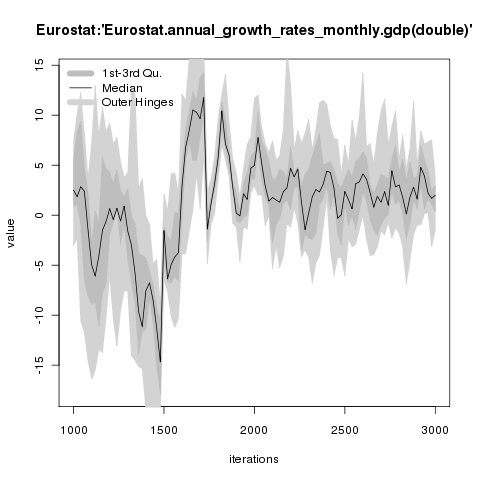
\includegraphics[width=8cm]{./energy_shock/png/duration_240/intensity_0.05/frequency_20/Eurostat-annual_growth_rates_monthly_gdp.png}
%\includegraphics[width=8cm]{./energy_shock/png/duration_240/intensity_0.05/frequency_20/Eurostat-total_subsidy_payment.png}
\end{minipage}
\caption{Effect of the stabilization policy in the energy shock experiment. Annualized growth rate and total subsidy payment by the government.}
\label{Figure: Stabilization}
\end{figure}
%\pagebreak 